%----------------------------------------------------------------------------------------
% Literature review
%----------------------------------------------------------------------------------------
\section{Models}
\subsection{Generalized Model}

We consider this generalized problem. Given a random variable $X$ with alphabet $\mathcal{X}$ and its distribution $p(x)$. We determine the value of $X$ by asking questions. The $i$-th question we ask is that "is $X$ in set $S_i$?", where $S_i \in \mathscr{A}, \forall i$. Suppose we need $N$ questions to determine the value of $X$. Our goal is to find out the minimum of $EN$ (the expectation of $N$) and if possible, its corresponding strategy.

\begin{definition}

The family of set $\mathscr{A}$ is called a decision set on $\mathcal{X}$.

\end{definition}

Obviously, different structures of the decision set will produce a bunch of completely different problems. In the rest of this chapter, we will introduce three specializations of this model, which are Huffman coding, the DNA detection problem and the Battleship problem.

\subsection{Huffman Coding: the Easy Case}

In Example \ref{badWine}, the decision set is $2^\mathcal{X}$. We have seen that in this case, the problem is equivalent to Huffman coding. However, the condition can be loosened slightly.

\begin{definition}

A decision set $\mathscr{A}$ on $\mathcal{X}$ is  decision-complete, if $\forall S\in 2^\mathcal{X} \setminus \{\emptyset, \mathcal{X}\}$, $S \in \mathscr{A} $ or $\mathcal{X} \setminus S \in \mathscr{A}$.

\end{definition}

\begin{proposition}
\label{decisionCompleteFeasible}
If $\mathscr{A}$ is decision-complete, then any decision tree of $X$ is feasible.
\end{proposition}

\begin{proof}
This is easy to demonstrate. Asking "is $X$ in set $S_i$?" is equivalent to asking "is $X$ in set $\mathcal{X} \setminus S_i$?", and there is no point to ask whether $X$ is in $\emptyset$ or $\mathcal{X}$.
\end{proof}

\begin{corollary}
\label{equivHuffman}
If $\mathscr{A}$ is decision-complete, then Huffman coding will produce the optimal solution.
\end{corollary}

% Corollary \ref{equivHuffman} tells us why Example \ref{badWine} is easy and Example \ref{moreBadWine} is hard. In Example \ref{badWine}, the decision set is decision-complete, so Huffman coding works. However, in Example \ref{moreBadWine}, we have seen that the decision set is no longer decision-complete, so Huffman coding might fail.

Proposition \ref{decisionCompleteFeasible} also provides a trivial but practical necessary condition for a set to be decision-complete.

\begin{corollary}
\label{minNumA}
If $\mathscr{A}$ is decision-complete, then $|\mathscr{A}| \ge 2^{|\mathcal{X}|-1} - 1$.
\end{corollary}

Using Corollary \ref{minNumA}, it is easy to prove that the decision set of Example \ref{moreBadWine} is not decision-complete,  so the Huffman coding strategy might fail.

\begin{proposition}
The decision set $\mathscr{A}$ of Example \ref{moreBadWine} is not decision-complete.
\end{proposition}

\begin{proof}
$|\mathcal{X}|=6$, so $|\mathscr{A}| = 2^4 - 1 < 2 ^{ |\mathcal{X}|-1} - 1$.
\end{proof}

\subsection{DNA Detection Problem}
To determine genomic sequences of several organisms, we need to assign biological meaning to particular regions of the sequence. One of important steps in this  process is the identification of genes. Exon is an interval of the DNA sequence and it does not overlap with other exons and gene is a sequence of exons. In this paper, we simplified the question by assuming that the target gene only contains one exon. We can detect whether the target exon is in an interval in the DNA sequence or not at each detection. The position of the exon on DNA is fixed, so we want to minimize the expected number of detection to determine the position of the exon by choosing the intervals wisely, thus reducing the cost of DNA detection\cite{biedl2004finding}\cite{xu1998gene}.

\begin{definition}
A set $S$ of integers is continuous, if $S = [\min S, \max S] \cap \mathbb{Z}$.
\end{definition}

\begin{example}
$\{1,2,3\}$ and $\{4\}$ are continuous, while $\{1,3\}$ is not.
\end{example}

If we assume that the exon's location we want to find on the DNA is discrete and unique, we can use a random variable $X\in \{1,2,\dots, n\}$ to it, and in this case, the decision set is any continuous set in space $\mathcal{X}$.

\begin{figure}
    \centering
    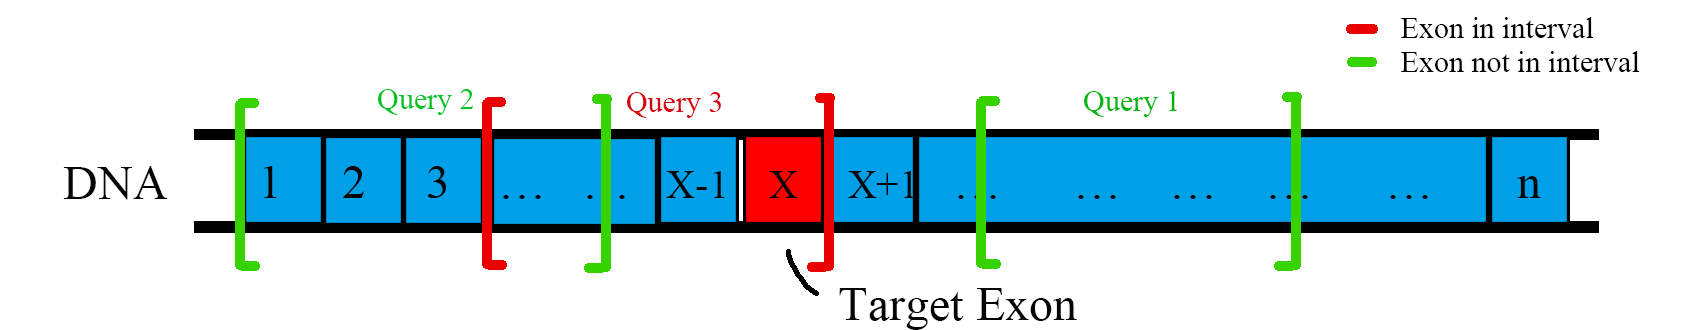
\includegraphics[width=0.9\textwidth]{figure/Exon.png}
    \caption{DNA exon detection.}
    \label{fig:exon}
\end{figure}

\subsection{Battleship Problem}
"Battleship" is a popular 2-player strategy and guessing game. In the typical setting, each player places "boats" with different lengths on his $10\times 10$ board, which is hidden to the opponent. Each player take turns to "bomb" a grid $(i,j)$ on opponent's board, and the opponent must honestly report if it "hits" or "misses". The goal of the game is sink all of the opponent's ships, i.e. "hit" all the grids on the opponent's board that represents a ship, before the opponent sinks all the player's ships. 
To simplify analysis and computation, we instead study the 1-player Battleship. In this setting, the game randomly generates a possible layout of ships unknown to the player. The goal of the player is to sink all the ships in the fewest tries (bombs). 
For example, in this particular board placed by the opponent (the game), the player needs to "hit" all grids marked in gray.
\begin{figure}[H]\label{battleshipgame}
    \centering
    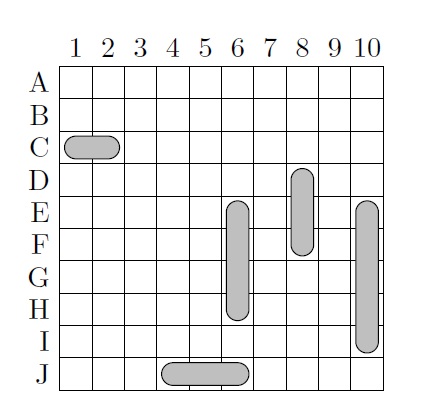
\includegraphics[scale=0.8]{figure/battleshipgame.png}
    \caption{One possible board of one player in Battleship
    \cite{battleshipoptimal}.}
\end{figure}

The 1-player Battleship problem can be formulated into the following. Suppose there are $n$ different possible ship layouts. Let $\mathcal{X}_0 = \{ X_1, X_2, X_3, \dots, X_n \}$ be the set of all possible layouts, where $X_k, 1\leq k \leq n$ is a $10\times 10$, $0-1$ matrix. The game randomly chooses the target board $X^{*} \in \mathcal{X}_0$ (every legal board is equally possible), and the player tries to minimize the number of tries $T$ to guess $T^{*}$.

At $t$-th step, the player gives a query on i, j: $Q_t  = (i_t,j_t)$, which means: "Is bombing of grid $(i,j)$ a hit?" the game answers honestly, giving the player some information to eliminate some layouts in $\mathcal{X}_{t-1}$ and get the new $\mathcal{X}_{t}$.
$$\mathcal{X}_t = \{X|(X\in \mathcal{X}_{t-1}) \wedge (X_{ij} = X^{*}_{ij})\}$$
The goal is to minimize the number of tries $T$ to determine what the target layout is,  by choosing queries wisely. That is, 

$$    \min_{Q_1, Q_2, \dots, Q_T} T  , Q_t = (i_t, j_t)$$
$$    \mathcal{X}_t = \{X|(X\in \mathcal{X}_{t-1}) \wedge (X_{i_t j_t} = X^{*}_{i_t j_t})\} , 1 \leq t \leq T$$
$$\mathcal{X}_0 = \{ X_1, X_2, X_3, \dots, X_n \},	\mathcal{X}_T = \{X^{*}\}, \text{ random variable } X^* \in \mathcal{X}_0 $$

More precisely, we would like to minimize the average number of tries $\bar{T}$ over all possible targets $X^{*}$.


Previous studies use diagonal searching\cite{Rodin}, tree search\cite{battleshipoptimal}, or RL-based\cite{battleshiprl} approaches. In our study, we adopt the idea of greedy information gain per step, which will be demonstrated in Chapter \ref{sec:gbsc}.



